%  
%  ICON - Fortran 2003 programming guide  
%  
%  - Luis Kornblueh, 13 Jan 2000, original version   
%  - Martin Schultz, 17 Jan 2000, English language corrections  
%  - Luis Kornblueh, 12 Apr 2000, change for introducing the DOCTOR naming   
%                                 standard and labeled do loops in the physics
%                                 package  
%  - Luis Kornblueh, 26 Jul 2000, changes recommended by Marco Giorgetta,  
%                                 added, section about parallelization and  
%                                 libraries added   
%  - Andreas Rhodin,   
%    Luis Kornblueh, 17 Aug 2000, description of parallelization  
%  - Martin Schultz, 17 Aug 2000, netCDF and parallel I/O   
%  
%  - Luis Kornblueh, 24 Mar 2004, updated for use within the ICON development
%  - Thomas Heinze,  10 May 2004, further updated for use within the ICON 
%                                 development    
%  - Thomas Heinze,  11 Aug 2004, included several minor features discussed  
%                                 at ICON meeting at MPI-M Hamburg:  
%                                 authors, Fortran 2003, date, DOCTOR style 
%  - Thomas Heinze,  21 Sep 2004, updated templates in appendix  
%                                 replaced MPIM by MPI-M   
%                                 replaced mo_kind.f90 by current version   
%                                 included mo_math_constants.f90
%  - Thomas Heinze,  28 Sep 2004, discarded IMPLICIT NONE in templates for
%                                 functions and subroutines  
%  - Thomas Heinze,  18 Jul 2005, cleaning up DOCTOR style
%                                 include latest mo_XX_constants  
%                                 include Peter Korn among authors  
%  - Thomas Heinze,  25 Jul 2005, include gnames_*.tex  
%                                 updated rules for variable names suggested
%                                 by M.Giorgetta
%  - Thomas Heinze,  26 Jul 2005, updated gnames_*.tex after DWD suggestions  
%                                 updated DOCTOR standard
%  - Thomas Heinze,  16 Aug 2005, updated global variable names
%  - Thomas Heinze,  29 Aug 2005, updated global variable names
%  - Thomas Heinze,  16 Feb 2006, clarified naming conventions for m_modules
%                                 and mo_modules
%  - Thomas Heinze,  22 Feb 2006, included updated templates
%  - Thomas Heinze,  22 Nov 2006, added latest compilers
%  - Luis Kornblueh, 05 Dec 2008, updated and proposed doxygen instead of incoprotex
%  - Luis Kornblueh, 23 Jun 2009, preprocessor defines
%  - Luis Kornblueh, 20 Jul 2009, changed form ProTeX to doxygen 
%  - Luis KOrnblueh, 21 Jul 2009, updated with change requests so far available
%  - Daniel Reinert, 21 Sep 2009, included section about OpenMP parallelization
%  - Daniel Reinert, 22 Sep 2009, changed documentation of global variable names 
%                                 (appendix)
% - Marco Giorgetta, 15 July 2010, Store section of the appendix on the grid structure in a 
%                                 separate file.
  
\documentclass[a4paper,11pt,DIV16,BCOR1cm,titlepage]{scrartcl}  

\usepackage[blocks]{authblk}
\usepackage{xcolor}  
\usepackage{listings}  
\usepackage{amsmath,amssymb}  
\usepackage{graphicx}  
\usepackage{tabularx} 
\usepackage{wrapfig}
\usepackage{array}
\usepackage{multirow}

\definecolor{darkgreen}{RGB}{0,119,112}  
\definecolor{darkgrey}{RGB}{209,206,198} 

\pagestyle{headings}  
  
\parindent 0pt  
\parskip 1ex plus 0.2ex minus 0.2ex  

\renewcommand{\ttdefault}{pcr}

\lstnewenvironment{fortran}%
{\lstset{language=[95]Fortran,%
basicstyle=\ttfamily\footnotesize\color{darkgreen},%
commentstyle=\ttfamily\color{blue},%
emptylines=0,%
keywordstyle=\color{black}\ttfamily\bfseries,%
backgroundcolor=\color{darkgrey!5},
framexleftmargin=4mm,%
frame=shadowbox,%
rulesepcolor=\color{darkgreen}}}
{}

\lstnewenvironment{lisp}%
{\lstset{language=lisp,%
basicstyle=\ttfamily\footnotesize\color{darkgreen},%
commentstyle=\ttfamily\color{blue},%
emptylines=0,%
keywordstyle=\color{black}\ttfamily\bfseries,%
backgroundcolor=\color{darkgrey!5},
framexleftmargin=4mm,%
frame=shadowbox,%
rulesepcolor=\color{darkgreen}}}
{}

\lstnewenvironment{csh}%
{\lstset{language=csh,%
basicstyle=\ttfamily\footnotesize\color{darkgreen},%
commentstyle=\ttfamily\color{blue},%
emptylines=0,%
keywordstyle=\ttfamily\footnotesize\color{darkgreen},%
backgroundcolor=\color{darkgrey!5},
framexleftmargin=4mm,%
frame=shadowbox,%
rulesepcolor=\color{darkgreen}}}
{}

\renewcommand\Affilfont{\itshape\normalsize}

\titlehead{  
\unitlength = 1mm  
\begin{picture}(80,0)  
\put(-10,-10){ 
\includegraphics[scale=0.3]{../resources/img/mpilogo.pdf} }  
\put(63,-20){\makebox(0,0)[rb]{\textbf{Max-Planck-Institut f\"ur Meteorologie}}}
\put(63,-24){\makebox(0,0)[rb]{Bundesstr. 53}}
\put(63,-29){\makebox(0,0)[rb]{D-20146 Hamburg}}
\end{picture}  
\hspace{1cm}
\begin{picture}(80,0)  
\put(50,-20){ 
\includegraphics[scale=0.6]{../resources/img/dwdlogo.pdf} }  
\put(5,-2){\makebox(0,0)[lb]{\textbf{Deutscher Wetterdienst}}}
\put(5,-7){\makebox(0,0)[lb]{Frankfurter Str. 135}}
\put(5,-11){\makebox(0,0)[lb]{D-63067 Offenbach}}
\end{picture}  
}  
  
\title{\vspace{6cm}ICON Grid Documentation}  
 
\author[1]{Leonidas Linardakis}
\author[2]{Daniel Reinert}
\author[1]{Almut Gassmann}
\affil[1]{Max-Planck-Institut f\"ur Meteorologie\\Bundesstr. 53\\D-20146 Hamburg\\Germany}   
\affil[2]{Deutscher Wetterdienst\\Frankfurter Str. 135\\D-63067 Offenbach\\Germany}  
  
\date{\vspace{8cm}\today}  
  
\begin{document}  

\maketitle  
  
\tableofcontents  
  
\newpage  

\section{The ICON spherical grid}
\label{sec:icon_spherical_grid}

%\begin{wrapfigure}{r}{0.5\textwidth}
\begin{figure}[!htd]
  \begin{center}
    \includegraphics[width=8.0cm,draft=false]{../contrib/ICON_earth_grid.jpg}
  \end{center}
  \caption{The ICON horizontal sphere grid. The light blue lines represent the projection of
    the original icosahedron edges. The dark blue lines depict the triangle grid
  after three edge bisections (R2B02). The black lines depict the dual hexagonal grid. 
  No optimization is applied.}
  \label{fig:icon_earth_grid}
\end{figure}
%\end{wrapfigure}

The ICON $3D$ spherical grid consists of two ``orthogonal'' components:
the horizontal grid,  and the vertical grid. 
The horizontal grid  discretizes the sphere surface, 
it is a triangular or a hexagonal grid, and 
it is described in Section \ref{sec:icon_horizontal_spherical_grid}.
The vertical dimension along the sphere radius
is discretized in by a set of horizontal layers, 
and is described in Section \ref{sec:icon_vertical_spherical_grid}.


\paragraph{Notation Notes:}
We distinguish between the physical (spatial) dimensions of a variable, which we denote 
by $nD$,  and the array dimensions that the variable is coded in, denoted by $kD_a$.
Variables that reside on a surface (the $xy$ coordinates) are $2D$ variables, 
while variables on the 3 space ($xyz$ coordinates) are $3D$.
In ICON the two types of dimensions $nD$ and $kD_a$ are not the same.

\paragraph{Coordinate systems:}
CG is an abbreviation for the \emph{geographical coordinates} (longitude - latitude). 
The associated data type is t\_geographical\_coordinates, defined in 
\linebreak src/shared/mo\_math\_utilities.f90 with members \%lon and  \%lat.

CC is an abbreviation for the $3D$ \emph{Cartesian coordinates}. 
In these coordinates the sphere is considered to be the unit sphere.
Unit tangent vectors on the sphere are invariant of the sphere radius length.
The associated data type is t\_Cartesian\_coordinates, defined in 
src/shared/mo\_math\_utilities.f90, with members \%x(3).

LC denotes the \emph{local zonal-meridional coordinate system}. 
A $2D$ local coordinate system is associated with
each point $P$ on the sphere surface , which spans the tangent plane at $P$.
The coordinates axes are aligned along the longitude and latitude curves 
through $P$.The associated data type is t\_tangent\_vectors, defined in 
src/shr\_horizontal/mo\_model\_domain.f90, with members \%v1 and \%v2.

\paragraph{Other Abbreviation Notes:}
ICON in some cases uses a specific \emph{orientation} convention in accessing the 
components or neigbors of the grid cells, edges and vertices. The orientation in 
most cases is counter clockwise, denoted by ccw. Clockwise orientation is denoted by cw.



\subsection{The ICON horizontal spherical grid}
\label{sec:icon_horizontal_spherical_grid}



The ICON horizontal spherical grid is based on the projection of the icosahedron on the sphere.
The initial icosahedron grid is refined by $n$-secting the edges, and further refinement 
is obtained by iteratively bisecting the created edges (see Fig. \ref{fig:icon_earth_grid}). 
In each iteration a grid optimization procedure can be applied. 
The naming convention for the ICON horizontal grid is R$n$B$k$\_\textit{optimization}, 
where $n$ is the number  of initial divisions of the icosahedron edges, 
$k$ is the number of bisecting iterations, 
and \textit{optimization} denotes the applied optimization.


\paragraph{Geometry:}
All lines in the ICON horizontal spherical grid are arcs of great circles.
Note that the normal and tangent vector at the edges form a left-handed coordinate system
(see Table  \ref{tbl:grid_edge_variables}).

\paragraph{Topology:} The connectivity is defined explicitly and can represent a general
unstructured grid.
For each grid entity a list of adjacent entities is stored. Most of these lists are ordered 
in a counter clockwise orientation. See Tables \ref{tbl:grid_cell_variables} to 
\ref{tbl:grid_vertex_variables} for more details.



\subsection{The ICON vertical grid}
\label{sec:icon_vertical_spherical_grid}

The vertical grid consists of a set of vertical layers.
Each of these layers carries the horizontal $2D$ grid 
structure, thus forming the $3D$ structure of the grid. 
The vertical coordinates have a terrain-following hybrid structure.
The hydrostatic dynamical core uses pressure-based vertical coordinates,
while the non-hydrostatic has height-based  vertical coordinates.
Details for the calculation of the vertical coordinates can be found in 
Hui Wan's Phd thesis \cite{HuiWanPhD}.


\section{ICON grid data and loop structures}
\label{sec:data_loop_structures}


The major ICON variables are mapped on the grid entities, 
namely on the grid cell centers, edge centers and vertices. 
Details on the the staggering scheme can be found in Section 
\ref{sec:triangular_model_structures}. 
In this section the data and loop structures are described.

\begin{figure}[!htd]
  \begin{center}
    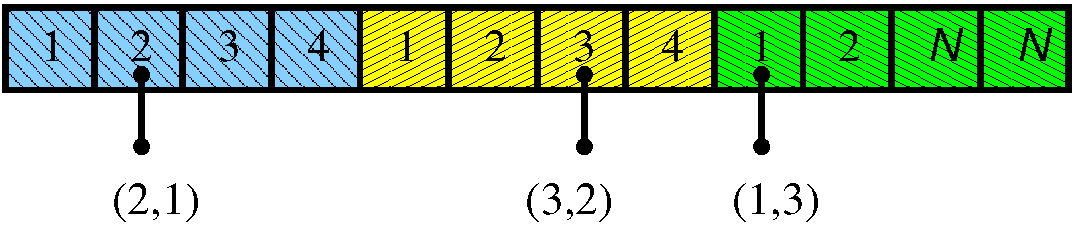
\includegraphics[width=10.0cm,draft=false]{../contrib/nproma_1.pdf}
  \end{center}
  \caption{Horizontal array structure with blocking factor $nproma=4$.
  The first index indicates the position inside the block, while the second index
  indicates the block. The last block contains 2 elements, the last two positions are 
  not used. The total memory size is 12, while the total number of elements is 10.}
  \label{fig:nproma_1}
\end{figure}


\begin{figure}[!htd]
  \begin{center}
    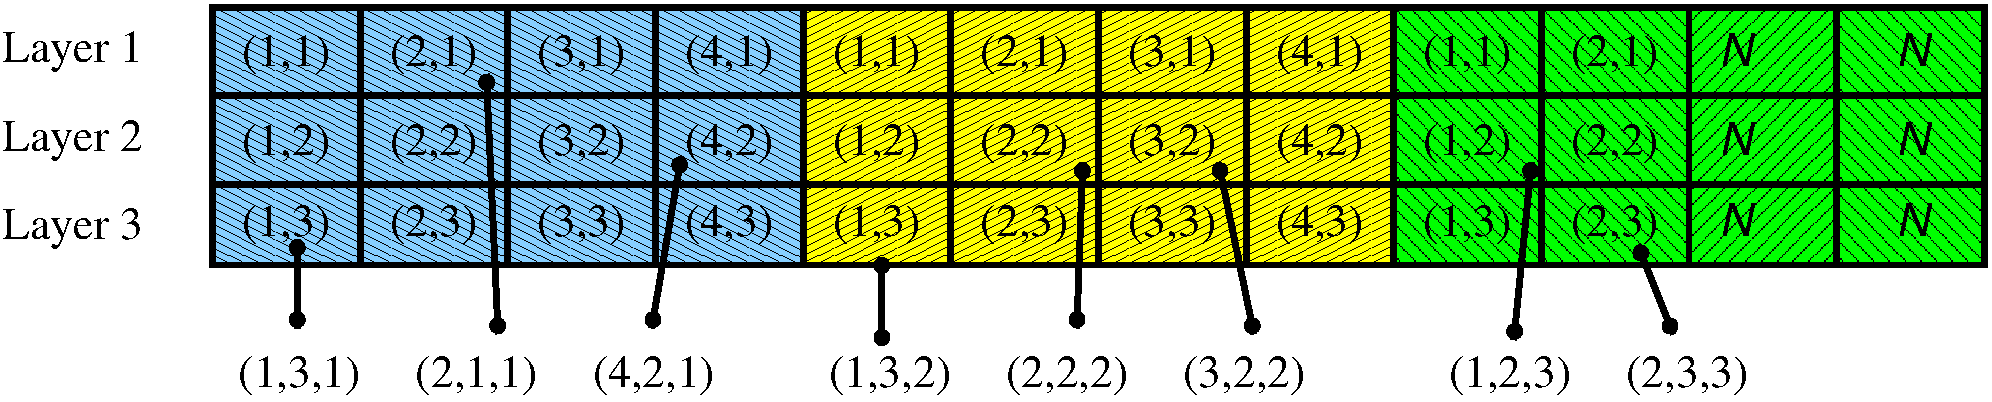
\includegraphics[width=16.0cm,draft=false]{../contrib/nproma_3d.pdf}
  \end{center}
  \caption{$3D$ array structure with blocking factor $nproma=4$ and three vertical layers.
  The first index indicates the position inside the block, the second the vertical layer, 
  the third index indicates the block. Each block occupies a continuous chunk of memory. 
  The last block contains 6 elements. 
  The total memory size is 36, while the total number of elements is 30.}
  \label{fig:nproma_3d}
\end{figure}


The horizontal grid data structure is designed to represent an 
unstructured grid and is mapped to one dimension. 
This single dimension is organized into blocks of $nproma$ size, 
resulting a two dimensional structure, with indices  
(index\_in\_block, block\_number), see Fig. \ref{fig:nproma_1}. 
$nproma$ is a constant, defined during runtime (see the ICON namelist description). 
The block size  may be different though on the array ``boundaries''.
This structure are designed to accommodate both vector 
and cache based architectures. A block of $nproma$ size can be processed 
as one vector by vector machines, or by one thread in a threaded environment.


$3D$ variables include an additional dimension representing the vertical layer
to which they belong, while maintaining the blocking structure in the horizontal dimension.
The indexing has the form (index\_in\_block, vertical\_layer, block\_number),
see Fig. \ref{fig:nproma_3d}. A typical $3D$ loop has the following structure.

\begin{fortran}
  DO jb = start_block, end_block
     CALL get_block_indices(p_patch, jb, start_block, end_block, &
                        i_startidx, i_endidx)
     DO jk = 1, vertical_layers
        DO je = i_startidx, i_endidx
            A(je,jk,jb) = ....
        ENDDO
    ENDDO
  ENDDO
\end{fortran}



\section{ICON triangular staggering scheme}
\label{sec:triangular_model_structures}

In ICON a C-staggering is applied to the triangular cells. Figure \ref{fig:hor_grid} and 
\ref{fig:vert_grid} show the location of all prognostic and the most important diagnostic 
variables in both horizontal and vertical directions. Table \ref{tbl:variables_nonhydro_model} 
provides a brief description of those variables, together with the variable names which are used 
in the code.
\begin{figure}[tbh]
  \begin{minipage}[t]{\linewidth}
    \begin{minipage}[t]{0.77\linewidth}
      \centering
      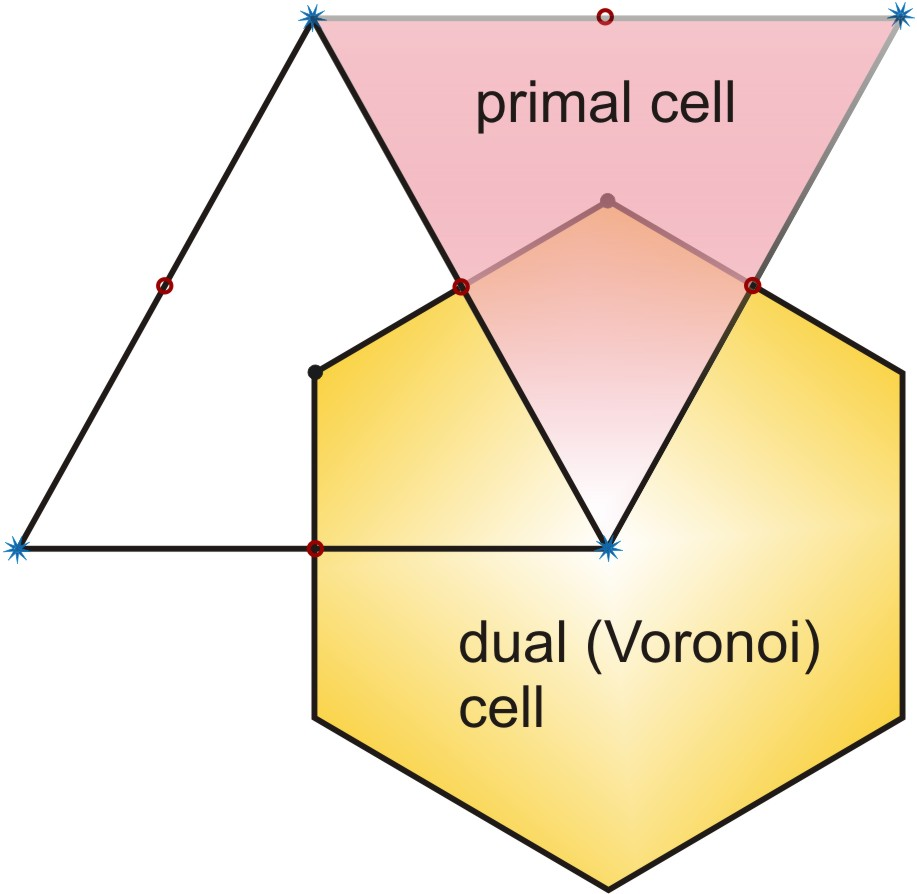
\includegraphics[width=6cm,draft=false]{../contrib/ICON_Grafik1_Okt09.jpg} %horizontal_grid}
    \end{minipage}
    \begin{minipage}[t]{0.2\linewidth}
      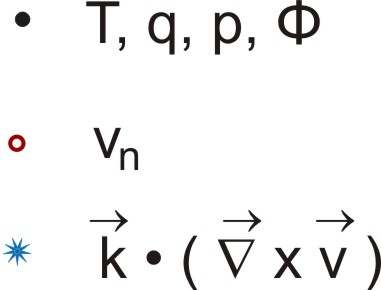
\includegraphics[width=3.0cm,draft=false]{../contrib/ICON_Grafik1_Legende_Okt09.jpg} %vertical_grid}
    \end{minipage}
    \caption{(a) Horizontal grid with primal cell (triangular) and dual cell (hexagonal). 
    Note that the dual edges are orthogonal to and bisect the primal edges.}\label{fig:hor_grid}
  \end{minipage}
%\end{figure}
%\begin{figure}[!h]
  \begin{minipage}[t]{\linewidth}
\vspace{0.4cm}
    \begin{minipage}[tbh]{0.77\linewidth}
      \centering
      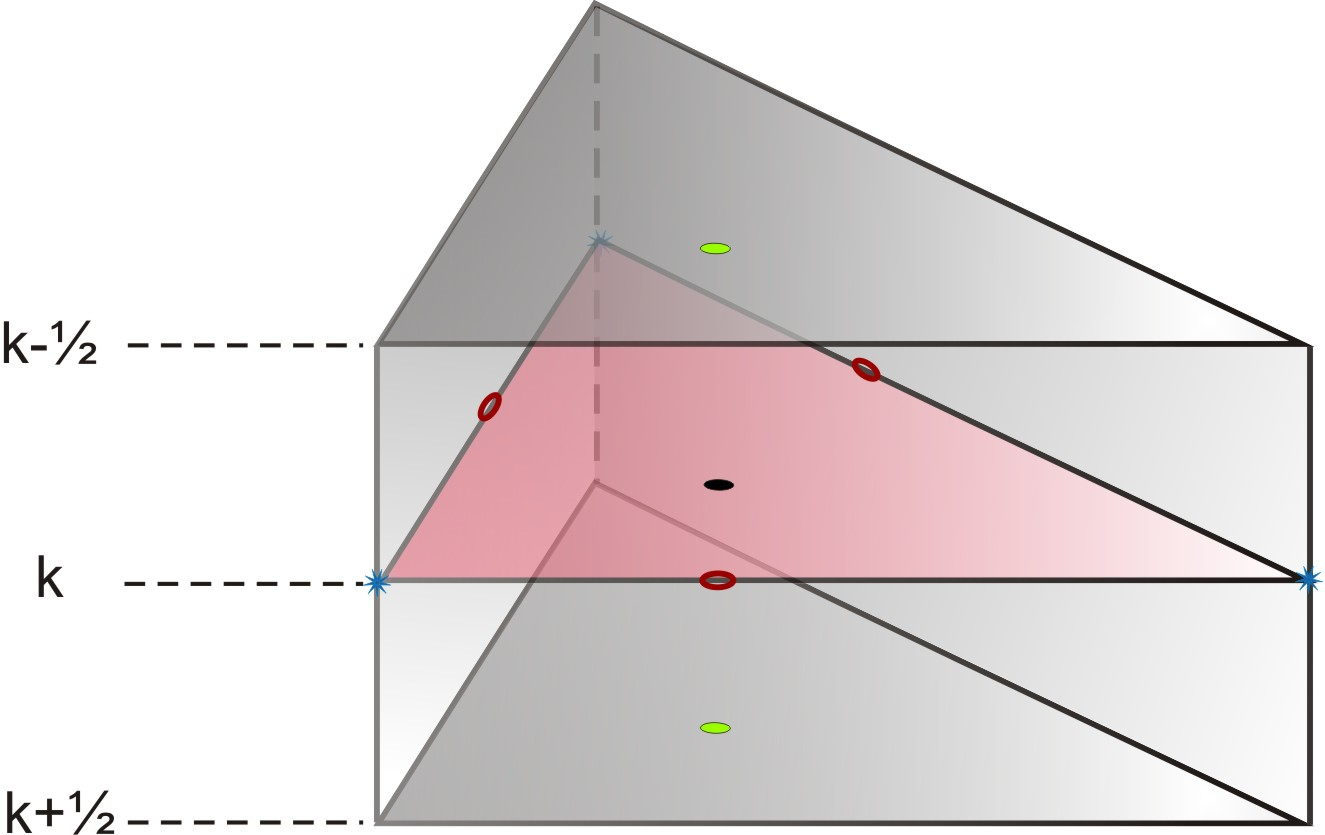
\includegraphics[width=7cm,draft=false]{../contrib/ICON_Grafik2_Okt09.jpg} %horizontal_grid}
    \end{minipage}
    \begin{minipage}[t]{0.2\linewidth}
      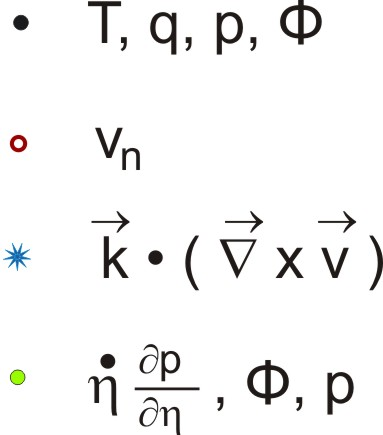
\includegraphics[width=3.cm,draft=false]{../contrib/ICON_Grafik2_Legende_Okt09.jpg} %vertical_grid}
    \end{minipage}
    \caption{Vertical structure of primal grid. The half levels ($k\pm 1/2$) correspond to $\eta$ 
    levels.}\label{fig:vert_grid}
  \end{minipage}
\end{figure}


\begin{table}[!h]
\renewcommand{\arraystretch}{1.4}
\small
\begin{center}
% use packages: array,tabularx
\begin{tabular}{|p{1.4cm}|p{2.9cm}|p{4.1cm}|p{4.4cm}|p{1.2cm}|}
\hline
\textbf{variable}  & \textbf{description}  &\textbf{position}         & \textbf{name within code}  & \textbf{unit}\\ 
\hline\hline
${\color{red}v_{n}}$    & normal velocity component  & edge midpoints of primal grid (full level)& $\mathrm{[hydro\_prog]\%vn(:,:,:)}$ & $m\,s^{-1}$\\ 
${\color{red}T}$        & temperature                & circumcenters of primal grid (full level)& $\mathrm{[hydro\_prog]\%temp(:,:,:)}$ & $K$\\ 
${\color{red}\theta}$   & potential temperature      & circumcenters of primal grid (full level)& $\mathrm{[hydro\_prog]\%theta(:,:,:)}$ & $K$\\
${\color{red}p_{s}}$    & surface pressure           & circumcenters of primal grid (half level)&  $\mathrm{[hydro\_prog]\%pres\_sfc(:,:)}$ & $Pa$\\
${\color{red}q}$        & scalar (i.e.\ mixing ratios) & circumcenters of primal grid (full level)& $\mathrm{[hydro\_prog]\%tracer(:,:,:,:)}$ & $kg\,kg^{-1}$\\
$\zeta$      & vertical component of relative vorticity  & vertices of primal grid (full level)& $\mathrm{[hydro\_diag]\%rel\_vort\_v(:,:,:)}$ &$ s^{-1}$\\ 
$\Phi$     & geopotential               & circumcenters of primal grid (full and half level)& $\mathrm{[hydro\_diag]\%geo\_mc(:,:,:)}$ & $m^{2}s^{-2}$\\
$\dot{\eta}\frac{\partial p}{\partial \eta}$ & vertical velocity ($\eta$ coord.) & circumcenters of primal grid (half level)&  $\mathrm{[hydro\_diag]\%weta(:,:,:)}$ & $Ps\,s^{-1}$\\
$\omega$ & vertical velocity (pressure coord.) & circumcenters of primal grid (half level)&  $\mathrm{[hydro\_diag]\%wpres(:,:,:)}$ & $Pa\,s^{-1}$\\
$u$                     & zonal velocity component   & circumcenters of primal grid (full level)& $\mathrm{[hydro\_diag]\%u(:,:,:)}$ & $m\,s^{-1}$\\ 
$v$                     & meridional velocity component   & circumcenters of primal grid (full level)& $\mathrm{[hydro\_diag]\%v(:,:,:)}$ & $m\,s^{-1}$\\
\hline
\end{tabular}
\caption{Overview of all prognostic and some diagnostic variables for the hydrostatic 
model. Prognostic variables are highlighted in red. Note: Only the most important 
diagnostic variables are listed here. For a complete list, see 
\texttt{src/hydro\_atmos/mo\_hydro\_state.f90}. The brackets in column $3$ indicate, that 
the prefix is a structure of type [\dots].}\label{tbl:variables_nonhydro_model}
\end{center}
\end{table}
\normalsize

The indexing of $2D$, $3D$ and $4D$ variables (fields) is as follows: For 2D fields, the second index 
(jb) relates to the block number and the first index ($jc$, $je$ or $jv$) relates to the position 
within the block. The label for the first index depends on whether the variable is defined at the 
cell center ($jc$), cell edge ($je$), or cell vertex ($jv$). For $3D$ fields, the block number ($jb$) 
is shifted to the third dimension. The second dimension ($jk$) now relates to the vertical level, 
where '1' is the top-most full (or half) level and 'nlev' ('nlev+1') is the lowest full 
(or half) level. For 4D fields (tracers), the first and second dimension are, again, the position 
within a block and the vertical level, respectively. The block number ($jb$) is shifted to the 
fourth dimension, while the third dimension ($jt$) relates to the tracer number.

Based on the above said, a specific value of a $2D$, $3D$, or $4D$ field at position 
($jc$) of block ($jb$) at level ($jk$) can be accessed as follows:
\begin{displaymath}
% use packages: array
\begin{array}{l l}
\text{2D:} &\mathrm{[hydro\_prog]\%pres\_sfc(jc,jb)} \\ 
\text{3D:} &\mathrm{[hydro\_prog]\%vn(jc,jk,jb)} \\ 
\text{4D:} &\mathrm{[hydro\_prog]\%tracer(jc,jk,jt,jb)}
\end{array}
\end{displaymath}


In Figure \ref{fig:grid_topology} the variables describing the grid topology 
and geometry are defined. In Table \ref{tbl_variables_grid_topology} these variables 
are briefly described and the names which are used in the code are listed.
\begin{figure}[htbp]
  \centering
  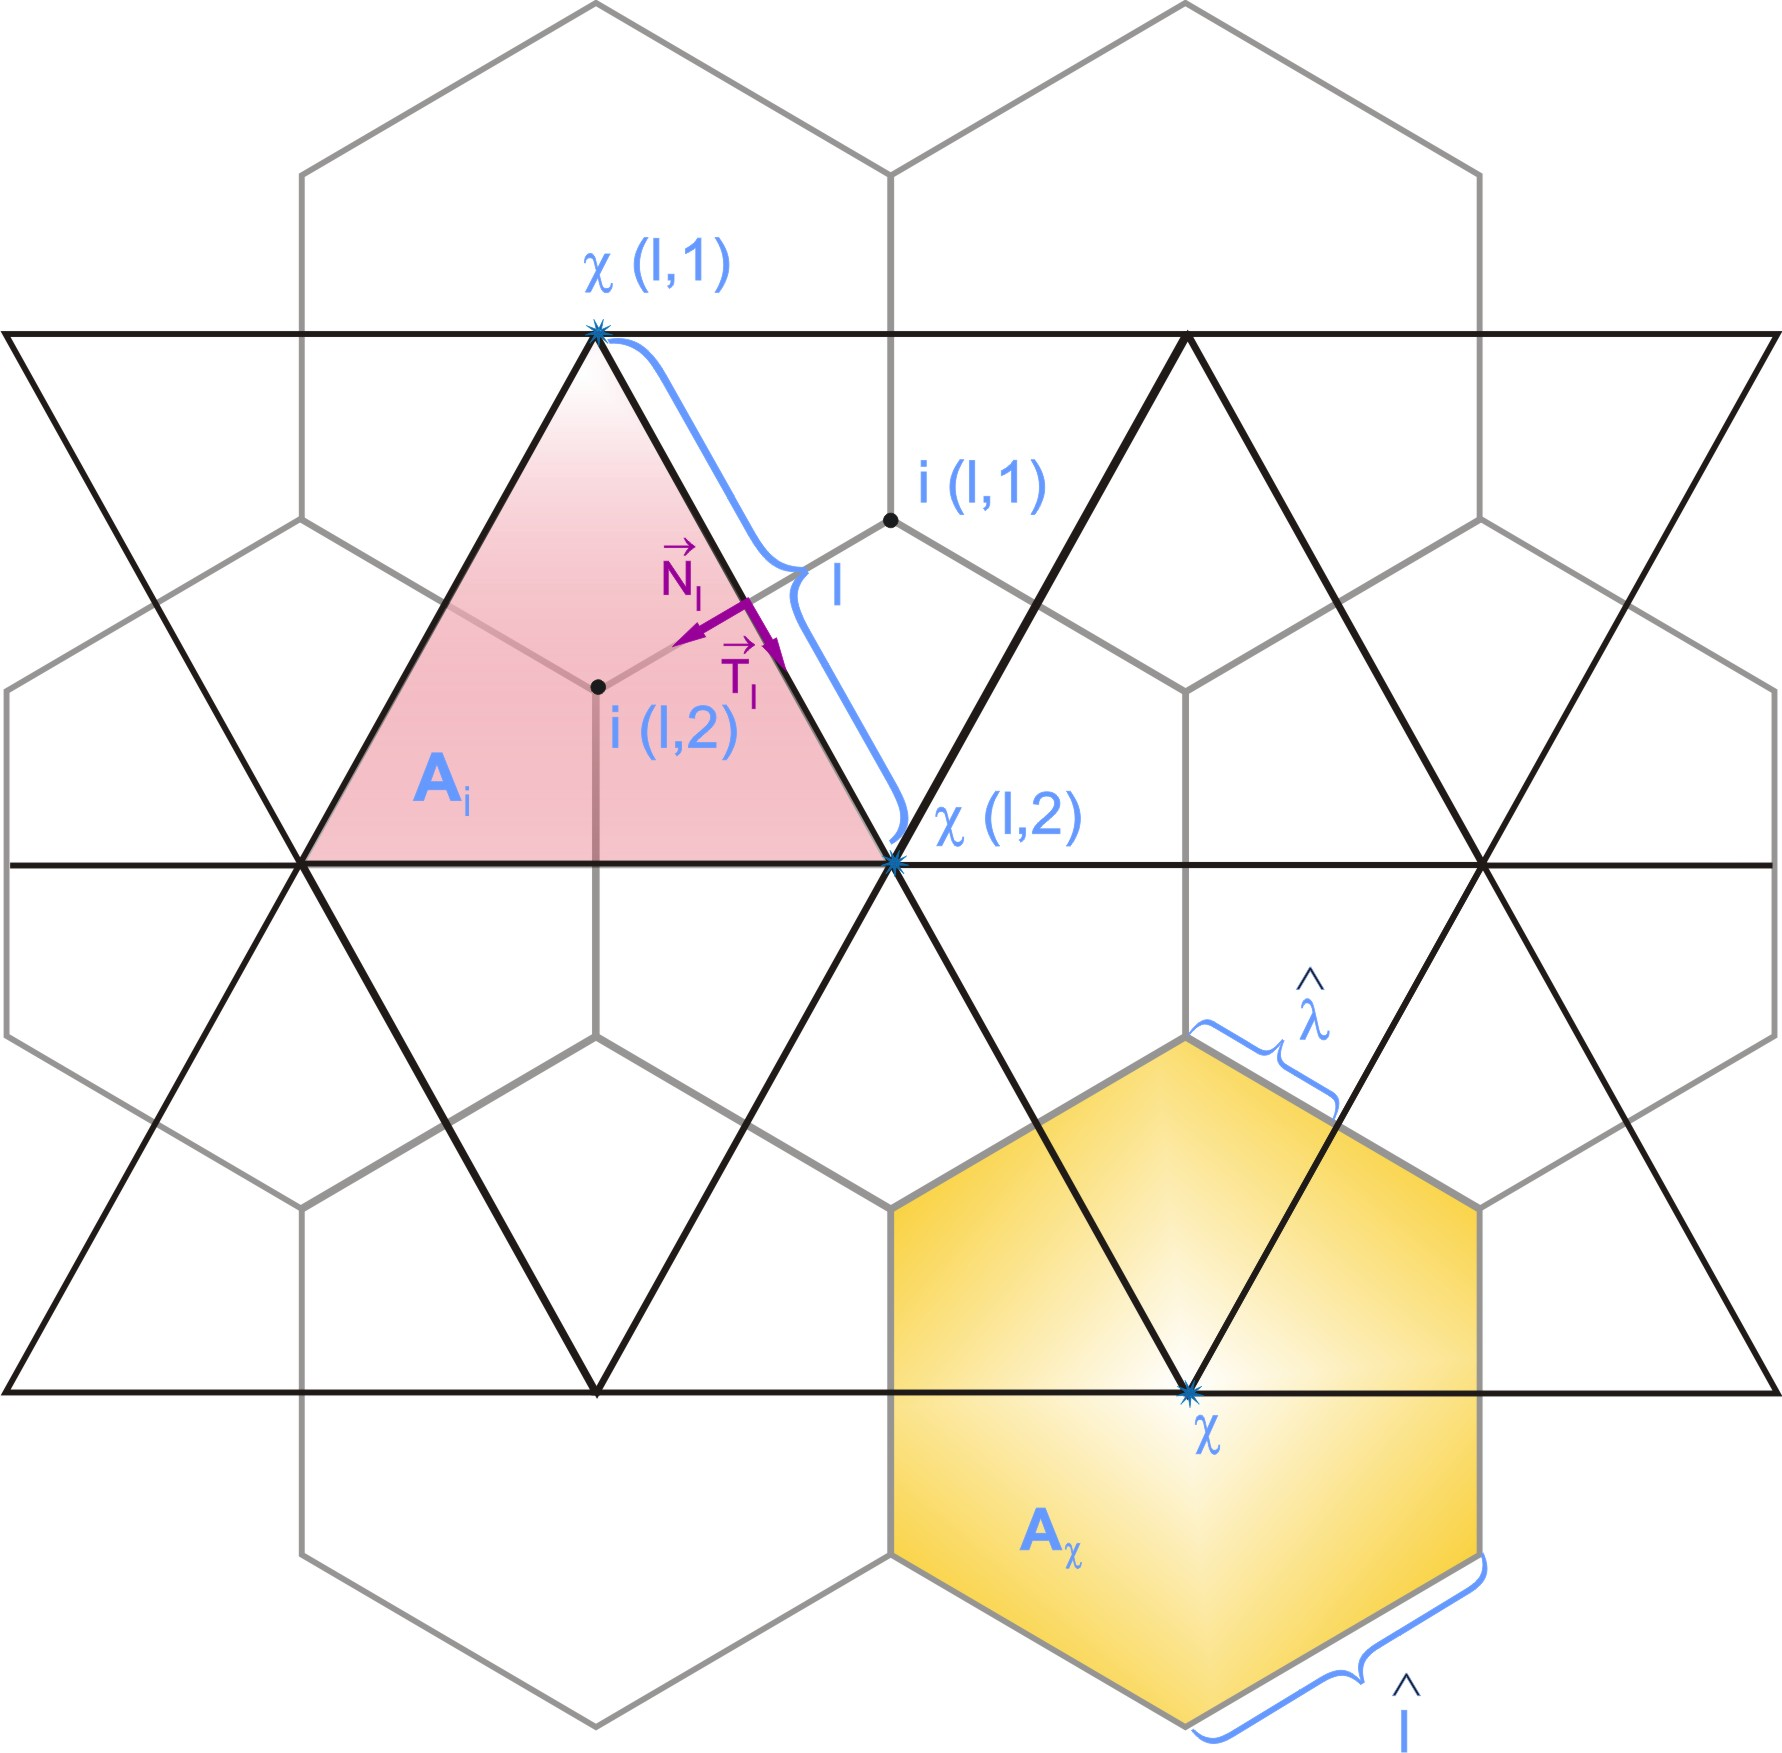
\includegraphics[width=7.0cm,draft=false]{../contrib/ICON_Grafik3_Okt09.jpg} %horizontal_grid}
    \caption{Notation for the horizontal grid. 
    See Table \ref{tbl_variables_grid_topology} for a description.}
    \label{fig:grid_topology}
\end{figure}

\begin{table}[!h]
\small
\renewcommand{\arraystretch}{1.4}
\begin{center}
% use packages: array,tabularx
\begin{tabular}{|p{2.2cm}|p{5.0cm}|p{6.5cm}|}
\hline
\textbf{variable}  & \textbf{description}  & \textbf{name within code} \\ 
\hline\hline
$i$              & triangular cell and its center         & [patch]\%cells\%idx(:,:) \\
$\chi$           & vertex of triangle and center of dual cell & [patch]\%verts\%idx(:,:)\\
$l$              & edge of triangular cell and its length & [patch]\%edges\%primal\_edge\_length(:,:) \\
$\hat{l}$        & edge of dual cell and its length       & [patch]\%edges\%dual\_edge\_length(:,:) \\
$\hat{\lambda}_{i,l}$  & distance between mass point $i$ and edge $l$ & [patch]\%edges\%edge\_cell\_length(:,:,:)\\
$A_{i}$          & Area of primal cell $i$                & [patch]\%cells\%area(:,:) \\
$A_{\chi}$       & Area of dual cell $\chi$               & [patch]\%verts\%dual\_area(:,:)\\
$N_{l}$          & Normal unit vector at edge $l$         & [patch]\%edges\%primal\_normal(:,:) \\
$T_{l}$          & Tangential unit vector at edge $l$     & [patch]\%edges\%dual\_normal(:,:)\\
$i(l,1), i(l,2)$ & the two neighboring triangles sharing edge $l$  & [patch]\%edges\%cell\_idx(:,:,:) \\
$\chi(l,1), \chi(l,2)$ & the two ends of edge $l$         & [patch]\%edges\%vertex\_idx(:,:,:)\\
\hline
\end{tabular}
\caption{List of symbols used for describing the horizontal grid. The brackets in column $3$ indicate, 
that the prefix is a structure of type \emph{patch}.}\label{tbl_variables_grid_topology}
\end{center}
\end{table}


\clearpage
\newpage

\appendix

\section{Grid Variables}

\begin{table}[htdp]
\small
\begin{center}
\begin{tabular}{|m{3.2cm}|m{3.3cm}|m{6.8cm}|m{1.6cm}|}
\hline
\multicolumn{4}{|c|}{\textbf{ICON grid cell variables}}\\ \hline
NETCDF         & name in the code        & description & (units,type,    \\ 
variable name  & [patch\%grid\_cells\%]  &             &  orientation)    \\ 
\hline\hline
neighbor\_cell\_ index  & neighbor\_[blk,idx](:,:,:)  & Index list of the neighbor cells & ccw\\
edge\_of\_cell  & edge\_[blk,idx](:,:,:)   & Index list of the cell edges    & ccw\\
vertex\_of\_cell& vertex\_[blk,idx](:,:,:) & Index list of the cell vertices & ccw\\
 & & & \\
orientation\_of\_normal & edge\_orientation(:,:,:) & 
The orientation of the edge normal vector (the variable primal\_normal in the edges table) 
for the cell according to Gauss formula.
It is equal to +1 if the normal to the edge is outwards from the cell, otherwise is -1.
The same is true for the tangent vectors and the Stokes formula
for a left-handed normal-tangent system (used in ICON).
& -1,+1,ccw \\
 & & &   \\
lon\_cell\_centre, lat\_cell\_centre & center(:,:) & lon, lat of cell centers & CG \\
 & & & \\
cell\_area\_p & area(:,:) & Area of cell & $m^2$ \\
\hline
\end{tabular}
\caption{Grid cell variables.}\label{tbl:grid_cell_variables}
\end{center}
\end{table}


\begin{table}[htdp]
\small
\begin{center}
\begin{tabular}{|m{3.2cm}|m{3.2cm}|m{6.8cm}|m{1.6cm}|}
\hline
\multicolumn{4}{|c|}{\textbf{ICON grid edge variables}}\\ \hline
NETCDF         & name in the code        & description & (units,type,    \\ 
variable name  & [patch\%grid\_edges\%]  &             &  orientation)    \\ 
\hline\hline
edge\_vertices  & vertex\_[blk,idx](:,:,:)  & Index list of the two edge vertices & \\
adjacent\_cell\_of\_edge  & cell\_[blk,idx](:,:,:)  & Index list of the two adjacent cells & \\
& & & \\
edge\_system\_\linebreak orientation  & system\_orientation(:,:)
& +1 if the vector from vertex(1) to vertex(2)
has the same orientation as the tangent vector (dual\_normal).
-1 otherwise.
& -1,+1\\
& & & \\
lon\_edge\_centre, lat\_edge\_centre & center(:,:) & lon, lat of the edge center & CG \\
& & & \\
zonal\_normal\_primal\_ edge \linebreak meridional\_normal\_\linebreak primal\_ edge
& primal\_normal(:,:)
& The normal (unit) vector to the edge in local coordinates
(on the tangent plane to the sphere).
It always points from cell(1) to cell(2). 
& LC \\
& primal\_cart\_normal
& The normal vector to the edge as above in Cartesian coordinates
& CC \\
& & & \\
zonal\_normal\_dual\_ edge \linebreak meridional\_normal\_\linebreak dual\_ edge
& dual\_normal(:,:)
& The tangent unit vector to the edge in local coordinates
(on the tangent plane to the sphere).
The primal\_normal, dual\_normal forms a left-handed coordinate system 
& LC \\
& dual\_cart\_normal
& The tangent unit vector to the edge, as above, in Cartesian coordinates
& CC \\
\hline
\end{tabular}
\caption{Grid edge variables.}\label{tbl:grid_edge_variables}
\end{center}
\end{table}


\begin{table}[htdp]
\small
\begin{center}
\begin{tabular}{|m{3.2cm}|m{3.3cm}|m{6.8cm}|m{1.6cm}|}
\hline
\multicolumn{4}{|c|}{\textbf{ICON grid vertex variables}}\\ \hline
NETCDF         & name in the code        & description & (units,type,    \\ 
variable name  & [patch\%grid\_vertices\%]  &          &  orientation)    \\ 
\hline\hline
vertices\_of\_vertex  & neighbor\_[blk,idx](:,:,:)  & Index list of the neighbor vertices         & (ccw)\\
cells\_of\_vertex  & cell\_[blk,idx](:,:,:)   & Index list of the cells containing this vertex    & (ccw)\\
edges\_of\_vertex  & edge\_[blk,idx](:,:,:)   & Index list of the edges containing this vertex    & (ccw)\\
 & & & \\
edge\_orientation & edge\_orientation(:,:,:) & 
+1 when the vector from this to the neighbor vertex has the same orientation as the 
tangent unit vector of the connecting edge.
-1 otherwise.
& -1,+1 \\
 & & &   \\
longitude\_vertices, longitude\_vertices & vertex(:,:) & lon, lat of the vertex & CG \\
 & & & \\
dual\_area\_p & dual\_area(:,:) & Area of the dual cell & $m^2$ \\
\hline
\end{tabular}
\caption{Grid vertex variables.}\label{tbl:grid_vertex_variables}
\end{center}
\end{table}

\clearpage
\newpage

\addcontentsline{toc}{section}{References}

\begin{thebibliography}{9}

  \bibitem{HuiWanPhD}
    Wan Hui, 
    \emph{Developing and testing a hydrostatic atmospheric dynamical core 
    on triangular grids}, PhD thesis, 
    Max Planck Institute for Meteorology,
    Hamburg, Germany,
    2009.

\end{thebibliography}
  
\end{document}  
  
  
